\\documentclass[titlepage,a4paper]{article}

\usepackage{a4wide}
\usepackage[colorlinks=true,linkcolor=black,urlcolor=blue,bookmarksopen=true]{hyperref}
\usepackage{bookmark}
\usepackage{fancyhdr}
\usepackage[spanish]{babel}
\usepackage[utf8]{inputenc}
\usepackage[T1]{fontenc}
\usepackage{graphicx}
\usepackage{float}

\pagestyle{fancy} % Encabezado y pie de página
\fancyhf{}
\fancyhead[L]{TP1S - Max Mustermann}
\fancyhead[R]{Algoritmos y Programación III - FIUBA}
\renewcommand{\headrulewidth}{0.4pt}
\fancyfoot[C]{\thepage}
\renewcommand{\footrulewidth}{0.4pt}

\begin{document}
\begin{titlepage} % Carátula
	\hfill
\includegraphics[width=6cm]{logofiuba.jpg}
    \centering
    \vfill
    \Huge \textbf{Trabajo Práctico 2 — AlgoRoma}
    \vskip2cm
    \Large [7507/9502] Algoritmos y Programación III\\
    Curso 2 \\ % Curso 1 para el de la tarde y 2 para el de la noche
    Segundo cuatrimestre de 2023 
    \vfill
    \begin{tabular}{ | l | l | } % Datos del alumno
      \hline
      Alumno 1: & Sosa, Juan Manuel \\ \hline
      \textit{Número de padrón:} & 92810 \\ \hline
      \textit{ Email:} & jmsosa@fi.uba.ar \\ \hline
      Alumno 2: & Maldonado Barbosa, Henry Mauricio \\ \hline
      \textit{Número de padrón:} & 99570 \\ \hline
      \textit{Email:} & hmaldonado@fi.uba.ar \\ \hline
      Alumno 3: & Servin Velazquez, Marcos \\ \hline
      \textit{Número de padrón:} & 101855 \\ \hline
      \textit{Email:} & maservin@fi.uba.ar \\ \hline
      Alumno 4: & Condori Zeballos, Favio Gustavo \\ \hline
      \textit{Número de padrón:} & 101906 \\ \hline
      \textit{Email:} & fcondori@fi.uba.ar \\ \hline
      Alumno 5: & Rodriguez, Nazareno Jose Luis \\ \hline
      \textit{Número de padrón:} & 101891 \\ \hline
      \textit{Email: }& nrodriguez@fi.uba.ar \\ \hline
  	\end{tabular}
    \vfill
    \vfill
\end{titlepage}




\tableofcontents % Índice general
\newpage

\section{Introducción}\label{sec:intro}
El presente informe reune la documentación de la solución del primer trabajo práctico de la materia Algoritmos y Programación III que consiste en desarrollar una aplicación de un sistema de una agencia de viajes en Pharo utilizando los conceptos del paradigma de la orientación a objetos vistos hasta ahora en el curso.

\section{Supuestos}\label{sec:supuestos}
% Deberá contener explicaciones de cada uno de los supuestos que el alumno haya tenido que adoptar a partir de situaciones que no estén contempladas en la especificación.

\begin{description}
    

\item[Supuesto] Lorem ipsum dolor sit amet, consectetur adipiscing elit. Proin nec facilisis odio. Pellentesque habitant morbi tristique senectus et netus et malesuada fames ac turpis egestas. In aliquam dapibus lacus at condimentum. Curabitur ornare scelerisque euismod. Duis a mi in nulla sodales sollicitudin vehicula sit amet sapien. Quisque vel eros ut libero consequat scelerisque. Nullam efficitur ante eu massa gravida sollicitudin.
\item[Supuesto] Curabitur elementum laoreet molestie. Ut hendrerit, quam lobortis porttitor cursus, ex sem facilisis massa, in interdum odio risus hendrerit dui.
\item[Supuesto] Integer porta efficitur felis. Etiam facilisis consectetur sem, ac efficitur orci. Nam a ante commodo, fringilla nisl a, sollicitudin est.

\end{description}

\section{Diagramas de clases}\label{sec:modelo}
% Varios diagramas de clases, mostrando la relación estática entre las clases. Pueden agregar todo el texto necesario para aclarar y explicar su diseño de manera tal que el modelo logre comunicarse de manera efectiva.

Donec fermentum volutpat diam, non sodales dui pulvinar nec. Vestibulum eu nisl lacus. Maecenas vel tortor efficitur, volutpat nulla id, ornare sem. Quisque nisi magna, vulputate sed purus eget, elementum volutpat velit.

\begin{figure}[H]
\centering
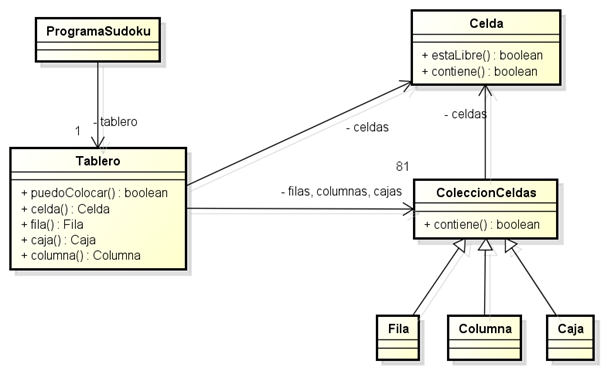
\includegraphics[width=0.8\textwidth]{ClasesDiagramas/diagrama_clase01.png}
\caption{\label{fig:class01}Diagrama del Sudoku.}
\end{figure}

Suspendisse sit amet feugiat nulla. Vivamus posuere sit amet diam condimentum sagittis. Sed et sapien in purus mattis ullamcorper sit amet non massa. Suspendisse tempus eleifend dapibus.

\section{Diagramas de secuencia}\label{sec:diagramasdeclase}
% Varios diagramas de secuencia, mostrando la relación dinámica entre distintos objetos planteando una gran cantidad de escenarios que contemplen las secuencias más interesantes del modelo.

Nunc molestie facilisis diam in auctor. Nulla sed porta nibh, eu elementum erat. Vestibulum in lectus ornare, sollicitudin ipsum eget, posuere risus. Duis ac ante sagittis, ornare urna a, scelerisque purus. Orci varius natoque penatibus et magnis dis parturient montes, nascetur ridiculus mus. Ut commodo ultricies luctus.

\begin{figure}[H]
\centering
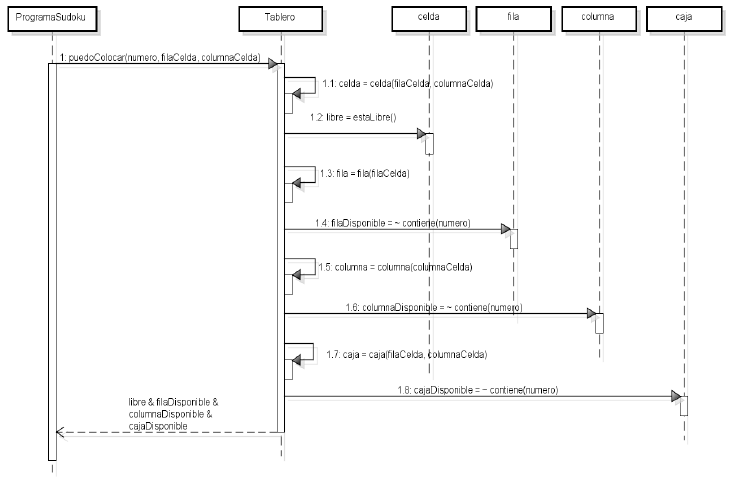
\includegraphics[width=\textwidth]{SecuenciasDiagramas/diagrama_secuencia02.png}
\caption{\label{fig:seq02}Nam a nulla non mauris ullamcorper.}
\end{figure}

In a elit malesuada, semper felis at, varius lorem. Aenean hendrerit vitae lorem sit amet porttitor. Suspendisse vitae vulputate elit, a commodo lacus. Phasellus maximus arcu et eros sollicitudin, eu aliquet nulla efficitur. Aenean semper neque nec dignissim rutrum. Aliquam at purus vel tortor fringilla iaculis sit amet sit amet metus. Pellentesque faucibus a nulla eget molestie.


\section{Diagrama de paquetes}\label{sec:implementacion}
% Incluir un diagrama de paquetes UML para mostrar el acoplamiento de su trabajo.

In a elit malesuada, semper felis at, varius lorem. Aenean hendrerit vitae lorem sit amet porttitor. Suspendisse vitae vulputate elit, a commodo lacus. Phasellus maximus arcu et eros sollicitudin, eu aliquet nulla efficitur. Aenean semper neque nec dignissim rutrum. Aliquam at purus vel tortor fringilla iaculis sit amet sit amet metus. Pellentesque faucibus a nulla eget molestie.


\section{Diagramas de estado}
% Incluir diagramas de estados, mostrando tanto los estados como las distintas transiciones para varias entidades del modelo.

In a elit malesuada, semper felis at, varius lorem. Aenean hendrerit vitae lorem sit amet porttitor. Suspendisse vitae vulputate elit, a commodo lacus. Phasellus maximus arcu et eros sollicitudin, eu aliquet nulla efficitur. Aenean semper neque nec dignissim rutrum. Aliquam at purus vel tortor fringilla iaculis sit amet sit amet metus. Pellentesque faucibus a nulla eget molestie.

\section{Detalles de implementación}
% Deben detallar/explicar qué estrategias utilizaron para resolver todos los puntos más conflictivos del trabajo práctico. Justificar el uso de herencia vs. delegación, mencionar que principio de diseño aplicaron en qué caso y mencionar qué patrones de diseño fueron utilizados y por qué motivos.

% IMPORTANTE No describir el concepto de herencia, delegación, principio de diseño o patrón de diseño. Solo justificar su utilización.

\subsection{Aliquam vel eros id magna vestibulum rhoncus}
Sed lorem diam, imperdiet in suscipit sed, lacinia id est. Duis ac turpis at velit tristique dictum ac in augue. Etiam porttitor purus sed nunc scelerisque aliquam. In hac habitasse platea dictumst. Mauris non mauris id lorem iaculis elementum eget quis mi.

\begin{verbatim}
| rango |
rango := (2 to: 20) asOrderedCollection.
Transcript show: rango ; cr.
rango copy do: [ :unNumero | unNumero isPrime ifFalse: [ rango remove: unNumero ] ].
Transcript show: rango.
\end{verbatim}

\subsection{Proin sodales leo dapibus sapien fermentum}
Quisque tempus, tortor et convallis interdum, ipsum leo tempus ipsum, in molestie tortor arcu sit amet tellus. Praesent fermentum hendrerit nulla. In maximus ornare maximus. Nullam consectetur placerat enim sit amet lacinia. Etiam pellentesque tellus consectetur hendrerit iaculis. Sed non laoreet felis.

\section{Excepciones}\label{sec:excepciones}
% Explicación de cada una de las excepciones creadas y con qué fin fueron creadas.

\begin{description}
% Explicar las excepciones creadas, con qué fin fueron creadas y cómo y dónde se las atrapa explicando qué acciones se toman al respecto una vez capturadas.

\item[Exception] Lorem ipsum dolor sit amet, consectetur adipiscing elit. Proin nec facilisis odio. Pellentesque habitant morbi tristique senectus et netus et malesuada fames ac turpis egestas. In aliquam dapibus lacus at condimentum. Curabitur ornare scelerisque euismod. Duis a mi in nulla sodales sollicitudin vehicula sit amet sapien. Quisque vel eros ut libero consequat scelerisque. Nullam efficitur ante eu massa gravida sollicitudin.
\item[Excepcion] Curabitur elementum laoreet molestie. Ut hendrerit, quam lobortis porttitor cursus, ex sem facilisis massa, in interdum odio risus hendrerit dui.
\item[Excepcion] Integer porta efficitur felis. Etiam facilisis consectetur sem, ac efficitur orci. Nam a ante commodo, fringilla nisl a, sollicitudin est.
\item[Excepcion] Aliquam erat volutpat. Fusce quis efficitur augue. Fusce egestas mauris a nisi finibus volutpat. Maecenas venenatis ligula ut nisi maximus, vel ultricies enim scelerisque.
\item[Excepcion] Mauris gatis feugiat erat non euismod. Donec sagittis orci enim, et convallis lacus sodales at. Nunc laoreet leo vel metus eleifend, vel aliquam sem tincidunt. Nunc imperdiet eget erat eget tincidunt. Morbi tempus risus quis nulla faucibus facilisis. Sed varius nunc vel neque rutrum vestibulum.
\end{description}

\end{document}

